%!TEX root = ../Thesis.tex
\section{Beschreibung des Projektverlaufs}

\subsection{Tatsächliche Aufgabenverteilung im Team (tabellarisch)}

\pagebreak

\subsection{Teammeeting-Protokolle}

{\def\arraystretch{1.25}\tabcolsep=5pt
\begin{longtable}{|l|l|p{11cm}|}
	\hline
	\textbf{Datum} & \textbf{Dauer} & \textbf{Beschreibung}
	\\ \hline \hline
	\endfirsthead
	
	\hline
	\endhead
	
	\hline
	\endfoot
	
	\multicolumn{3}{|c|}{\textit{Summe der Dauer aller Gruppenmeetings: 1.180 Minuten}}
	\\ \hline
	\multicolumn{3}{|c|}{\textit{Summe der Dauer aller GUI-Team-Meetings: 1.020 Minuten}}
	\\ \hline
	\multicolumn{3}{|c|}{\textit{Summe der Dauer aller Architektur-Team-Meetings: 360 Minuten}}
	\\ \hline
	\multicolumn{3}{|c|}{\textit{Summe der Dauer aller GUI-Team-Meetings: 110 Minuten}}
	\\ \hline
	\endlastfoot
	
		\textbf{03.09.2019} 
			& \textbf{200 Min.} & \textbf{Gruppenmeeting 1 - Projektauswahl}
			\\ & &
			\small{\textit{Teilnehmer: Bockhorn, Falk, Gentges, Istogu, Keienburg, Meinerzhagen, Pham, Schwenke}}
			\\ & &
			Auswahl des Projekttyps. Entscheidung für die Entwicklung einer Android-App.
			\\ & &
			Erste Einarbeitung in die Thematik. Lesen des bereitgestellten Dokuments mit Aufgabenstellung, groben Anforderungen und organisatorisches. 
			\\ & &
			Konzepterarbeitung auf Papier. Vorstellung und Diskussion verschiedener Ansätze.
	\\\hline
		\textbf{04.09.2019} 
			& \textbf{110 Min.} & \textbf{Gruppenmeeting 2 - Grobes Konzept}
			\\ & &
			\small{\textit{Teilnehmer: Bockhorn, Falk, Gentges, Istogu, Keienburg, Meinerzhagen, Pham, Schwenke, Herr Prof. Dr. Seifert}}
			\\ & &
			Einigung mit dem Dozenten auf einen Ansatz für den Taschenrechner.
			\\ & &
			Absprachen über Meeting-Protokolle, Studienarbeit und Projekttagebücher
			\\ & &
			Ausarbeitung des Konzepts für den Taschenrechner. Hier wurden dem Auftraggeber Herr Seifert mehrere Konzepte vorgestellt und gemeinsam mit ihm genaue Anforderungen erarbeitet.
			\\ & &
			Aufteilung der Gruppe in das GUI-, Architektur- und Backend Team
	\\\hline
		\textbf{05.09.2019} 
			& \textbf{60 Min.} & \textbf{GUI-Team-Meeting 1 - Prototyp} 
			\\ & &
			\small{\textit{Teilnehmer: Bockhorn, Gentges, Pham}}
			\\ & &
			Erstellung des Mid-Fidelity Prototypen in Power Point.			
		\\ \cline{2-3}
		& \textbf{60 Min.} & \textbf{Architektur-Team-Meeting 1 - Konzept} 
			\\ & &
			\small{\textit{Teilnehmer: Falk, Meinerzhagen, Schwenke}}
			\\ & &
			Grobe Konzeptionierung der Architektur des Projektes inklusive grobem Aufbau des Projektes und der Schnittstellen  
		\\ \cline{2-3}
		& \textbf{60 Min.} & \textbf{Backend-Team-Meeting 1 - Funktionen sammeln} 
			\\ & &
			\small{\textit{Teilnehmer: Istogu, Keienburg}}
			\\ & &
			Brainstorming über geplante Operatoren, Operanden und Einstellungen
		\\ \cline{2-3}
		& \textbf{60 Min.} & \textbf{Gruppenmeeting 3 - Abstimmung der Teams} 
			\\ & &
			\small{\textit{Teilnehmer: Bockhorn, Falk, Gentges, Istogu, Keienburg, Meinerzhagen, Pham, Schwenke}}
			\\ & &
			Besprechung des aktuellen Stands der Architektur, der Backend-Ideen und des Prototypen.
			\\ & &
			Diskussion über Umsetzung und Workflow der App.
			\begin{itemize}\renewcommand\labelitemi{--}
				\item  Wie sollen die einzelnen Kacheln funktionieren?
				\item Wie sollen die Kacheln miteinander interagieren?
				\item Wie könnte die Architektur der App aussehen?
			\end{itemize}
			\\ & &
			Absprache der Projektplanungsergebnisse
	\\\hline
		\textbf{13.09.2019} 
			& \textbf{ 120 Min.} & \textbf{GUI-Team-Meeting 2 - Mid-Fidelity Prototyp} 
			\\ & &
			\small{\textit{Teilnehmer: Bockhorn, Gentges, Pham}}
			\\ & &
			Erweiterung des Mid-Fidelity Prototyps in PowerPoint inlusive Workflow mit Links
			\\ & &
			Finalisierung der geplanten Funktionalitäten des Prototypen
	\\\hline
		\textbf{17.09.2019} 
			& \textbf{ 60 Min.} & \textbf{Architektur-Team-Meeting 2 - Klassendiagramm}
			\\ & &
			\small{\textit{Teilnehmer: Falk, Istogu, Meinerzhagen, Schwenke}}
			\\ & &
			Erweiterung UML-Klassendiagramm. Die Klasse Operand wird abstrakt und wird von konkreten Operanden wie Vector geerbt. Diese stellen Extensions dar die neben den eigentlichen mathematischen Werten weitere Daten und Verhalten mitbringen.
			\\ & &
			Welche Library soll für Mathe-Funktionalitäten benutzt werden? JScience und die bereits mitgelieferte Standardbibliothek.
			\\ & &
			Darstellungsformen der Elemente mit ASCI-Art oder LaTeX
		\\ \cline{2-3}
		& \textbf{90 Min.} & \textbf{GUI-Team-Meeting 3 - Workflow} 
			\\ & &
			\small{\textit{Teilnehmer: Bockhorn, Gentges, Pham}}
			\\ & &
			Wie sollen Elemente in der GUI dargestellt werden? Als Character oder gerendert in LaTeX. Letzteres ist mit höherer Komplexität verbunden sieht aber auch besser aus. 
			\\ & &
			Wie soll das Layout funktionieren? Gridlayout fällt raus, weil nicht dynamisch genug? Relative-Layout ist eine Option. Hier darf aber die Anordnung beim Rotieren nicht unkontrolliert verändert werden. UI Team möchte, dass alle Komponenten gleich groß sind. In dem Fall kann man Gridlayout benutzen.
			\\ & &
			Wie soll die Eingabe von Funktionen im Graph Operand funktionieren? Nur möglich mit bereits vorhandenen Elementen in der Oberfläche. Es öffnet sich keine Tastatur.
	
	\\\hline
		\textbf{23.09.2019} 
			& \textbf{ 120 Min.} & \textbf{GUI-Team-Meeting 4 - Prototyp} 
			\\ & &
			\small{\textit{Teilnehmer: Bockhorn, Gentges, Pham}}
			\\ & &
			Finalisierung des Mid-Fidelity Prototyps inklusive der Funktionalitäten
			\\ & &
			Durchplanung des Workflows			
	\\\hline
		\textbf{26.09.2019} 
			& \textbf{ 150 Min.} & \textbf{Gruppenmeeting 4 - Abstimmung der Teams}
			\\ & &
			\small{\textit{Teilnehmer: Bockhorn, Falk, Gentges, Istogu, Keienburg, Meinerzhagen, Pham, Schwenke}}
			\\ & &
			Vorstellung des Mid-Fidelity Prototyps und Einholung von Feedback
			\\ & &
			Erklärung der geplanten Systemarchitektur
			\\ & &
			Darstellung der geplanten Programmodule			
	\\\hline
		\textbf{09.10.2019} 
			& \textbf{90 Min.} & \textbf{Gruppenmeeting 5 - Abstimmung der Teams}
			\\ & &
			\small{\textit{Teilnehmer: Bockhorn, Falk, Gentges, Istogu, Keienburg, Meinerzhagen, Pham, Schwenke}}
			\\ & &
			Vorstellung des Backend-Entwurfs für Teammitglieder, die für das Frontend zuständig sind.
			\\ & &
			Vorstellung des Frontend-Entwurfs für Teammitglieder, die für das Backend zuständig sind.
			\\ & &
			Diskussion über Verbindung von Frontend und Backend. Wie abgekoppelt lässt sich der Calculator wirklich realisieren?
			\\ & &
			Vorstellung der Hauptbibliothek die für die (aufwändigen) Rechnungen wie Nullstellenberechnung benutzt werden soll.
			\\ & &
			Warum Apache Commons Math und nicht JScience?
			\\ & &
			Diskussion des Programm-Workflows.
	\\ \hline
		\textbf{05.01.2020} 
			& \textbf{120 Min.} & \textbf{Gruppenmeeting 6 - Abstimmung der Teams}
			\\ & &
			\small{\textit{Teilnehmer: Bockhorn, Falk, Gentges, Istogu, Keienburg, Meinerzhagen, Pham, Schwenke}}
			\\ & &
			Aufnahme des aktuellen Projektstands.
			\\ & &
			Besprechung des weiteren Vorgehens.
			\\ & &
			Abstimmung de Aufgaben.
			\\ & &
			Besprechung des geplanten Frontends.
			\\ & &
			Besprechung / Lösung von Problemen.
		\\ \cline{2-3}
		& \textbf{180 Min.} & \textbf{GUI-Team-Meeting 5 - Abstimmung der Teams} 
			\\ & &
			\small{\textit{Teilnehmer: Bockhorn, Gentges, Pham}}
			\\ & &
			Besprechung des Frontends und Einarbeitung des Feedbacks
			\\ & &
			Recherche nach Emulator Skins
			\\ & &
			Erste Drafts des Layouts
			\\ & &
			Anlegen der Kacheln (Style resource)	
	\\ \hline
		\textbf{10.01.2020} 
			& \textbf{90 Min.} & \textbf{GUI-Team-Meeting 6 - Layouts}
			\\ & &
			\small{\textit{Teilnehmer: Bockhorn, Gentges, Pham}}
			\\ & &
			Weitere Standardlayouts finalisiert
			\\ & &
			Kachelarchitektur für Frontend finalisiert			
	\\ \hline
		\textbf{14.01.2020} 
			& \textbf{90 Min.} & \textbf{Gruppenmeeting 7 - Integration der Komponenten}
			\\ & &
			\small{\textit{Teilnehmer: Bockhorn, Falk, Gentges, Istogu, Keienburg, Meinerzhagen, Pham, Schwenke}}
			\\ & &
			Zusammenführung Frontend Backend
			\\ & &
			Präsentation des Frontends durch das GUI-Team.
			\\ & &
			Besprechen von MVP-Umsetzung in Android.
			\\ & &
			Backend Unit-Testing Fortschritte.
			\\ & &
			Serialisierung der Stacks zur Session-Sicherung.
	\\ \hline
		\textbf{24.01.2020} & 
			\textbf{240 Min.} & \textbf{Architektur- und Backend-Team-Meeting}
			\\ & &
			\small{\textit{Teilnehmer: Falk, Istogu, Keienburg, Meinerzhagen, Schwenke}}
			\\ & &
			Detaillierte Ausarbeitung der Architektur im Backend.
			\\ & &
			Programmieren im Team inklusive der Zusammenführung der Features
			\\ & &
			Umbau der Programmstruktur zur Anpassung an MVP
	\\ \hline
		\textbf{28.01.2020} 
			& \textbf{90 Min.} & \textbf{Prototyp Vorstellung}
			\\ & &
			\small{\textit{Teilnehmer: Bockhorn, Falk, Istogu, Meinerzhagen, Schwenke Herr Prof. Dr. Seifert}}
			\\ & &
			Gespräch mit Herr Prof. Dr. Thomas Seifert über den aktuellen Stand des Projekts und im Anschluss daran eine Nachbesprechung innerhalb des Teams.
			\\ & &
			Vorstellung:
			\begin{itemize}\renewcommand\labelitemi{--}
				\item Vorstellung der bereits implementierten Grundfunktionen der App.
				\item Vorstellung des verwendeten Design-Patterns.
				\item Abgleich von Umsetzung mit den Anforderungen des Dozenten.
				\item Ansatz des Backends erklärt.
				\item Gerät ausleihen, um nicht nur mit Emulator testen zu können.
				\item Serialisierung der Daten (Speichern und Laden).
			\end{itemize}
			\\ & &
			Ergebnis:
			\begin{itemize}\renewcommand\labelitemi{--}
				\item Projekt ist auf einem guten Weg. Priorisiert werden sollen differenzierende Funktionen anstatt wenige Features sehr detailliert auszuarbeiten (Prototypische Arbeit).
				\item Ternäre, Quaternäre usw. Operationen sind gewünscht.
				\item Vektoren in Bestandteile lösen.
				\item Eingabe von Matrizen.
				\item Jeder Klasse muss ein Verantwortlicher zugeordnet sein.
			\end{itemize}		
		\\ \cline{2-3}
		& \textbf{90 Min.} & \textbf{Gruppenmeeting 8 - Nachbesprechung Vorstellung}
			\\ & &
			\small{\textit{Teilnehmer: Bockhorn, Falk, Gentges, Istogu, Keienburg, Meinerzhagen, Pham, Schwenke}}
			\\ & &
			Ergebnisse der Nachbesprechung
			\begin{itemize}\renewcommand\labelitemi{--}
				\item ''Vektor bauen'' / ''Vektoren auflösen'' Action. 
				\item Summe von Stack Action.
				\item 1x Triple Operator einfügen.
				\item Operanden Eingabe via einzelne Menüs.
				\item Ranks der Stacks anpassen.
				\item Format des ersten Stacks anpassen.
			\end{itemize}
		\\ \cline{2-3}
		& \textbf{120 Min.} & \textbf{GUI-Team-Meeting 7 - Tests \& Menüs } 
			\\ & &
			\small{\textit{Teilnehmer: Bockhorn, Gentges, Pham}}
			\\ & &
			Funktionstests des Frontends 
			\\ & &
			Beginn der Implementierung der Menüführung			
	\\ \hline
		\textbf{03.02.2020} 
			& \textbf{90 Min.} & \textbf{Gruppenmeeting 9 - Absprachen \& Dokumentation}
			\\ & &
			\small{\textit{Teilnehmer: Bockhorn, Falk, Gentges, Istogu, Keienburg, Meinerzhagen, Pham, Schwenke}}
			\\ & &
			Besprechen des aktuellen Stands der App.
			\\ & &
			Was muss noch unbedingt umgesetzt werden?
			\\ & &
			Aufteilung der noch offenen Kapitel in der Ausarbeitung.
			\\ & &
			Neues Kapitel ''Einleitung'' mit Motivation.
			\\ & &
			Anpassung einiger Kapitelbezeichnungen an Gegebenheiten des Projekts.
			\\ & &
			Koordination der Ausarbeitung.
		\\ \cline{2-3}
		& \textbf{50 Min.} & \textbf{Backend-Team-Meeting 2 - Finalisierung}
			\\ & &
			\small{\textit{Teilnehmer: Istogu, Keienburg}}
			\\ & &
			Absprache der letzten zu anzupassenden Funktionalitäten
	\\ \hline
		\textbf{05.02.2020} 
			& \textbf{90 Min.} & \textbf{Gruppenmeeting 10 - Finalisierung \& Dokumentation}
			\\ & &
			\small{\textit{Teilnehmer: Bockhorn, Falk, Gentges, Istogu, Keienburg, Meinerzhagen, Pham, Schwenke}}
			\\ & &
			Ergebnisbesprechung für das App-Debugging.
			\\ & &
			Gemeinsames Arbeiten an der Dokumentation.
	\\ \hline
\end{longtable}
}

\subsection{Projekttagebücher}

\subsubsection{Tom Bockhorn}

\subsubsection{Hendrik Falk}

\subsubsection{Dennis Gentges}

\subsubsection{Getuart Istogu}
{\def\arraystretch{1.25}\tabcolsep=5pt
	\begin{longtable}{|l|l|p{11cm}|}
		\hline
		\textbf{Datum} & \textbf{Dauer} & \textbf{Beschreibung}
		\\ \hline \hline
		\endfirsthead
		
		\hline
		\endhead
		
		\hline
		\endfoot
		
		\multicolumn{3}{|c|}{\textit{Summe der Dauer aller Aktivitäten: 4.370 Minuten}}
		\\ \hline
		\endlastfoot
		
		\textbf{03.09.2019} 
		& \textbf{200 Min.} & Gruppenmeeting 1
		\\ \hline
		
		\textbf{04.09.2019} 
		& \textbf{110 Min.} & Gruppenmeeting 2
		\\ \hline
		
		\textbf{04.09.2019} 
		& \textbf{40 Min.} & Ideen für mögliche Operatoren und Operanden sammeln
		\\ \hline
		
		\textbf{04.09.2019} 
		& \textbf{10 Min.} & Offizielle und interne Deadlines in Planner eintragen
		\\ \hline
		
		\textbf{05.09.2019} 
		& \textbf{60 Min.} & Gruppenmeeting 3
		\\ \hline
		
		\textbf{05.09.2019} 
		& \textbf{60 Min.} & Backend-Team-Meeting 1
		\\ \hline
		
		\textbf{17.09.2019} 
		& \textbf{60 Min.} & Architektur-Team-Meeting 2
		\\ \hline
		
		\textbf{26.09.2019} 
		& \textbf{150 Min.} & Gruppenmeeting 4
		\\ \hline
		
		\textbf{09.10.2019} 
		& \textbf{90 Min.} & Gruppenmeeting 5
		\\ \hline
		
		
		\textbf{12.10.2019} 
		& \textbf{30 Min.} & 
				Ermitteln der benötigten Operanden-Klassen (z.B. Matrix etc.) \\ & &
				
				Ermitteln der benötigten Operatoren-Klassen (Addition, Multiplikaiton usw.)
		\\ \hline
		
		\textbf{26.10.2019} 
		& \textbf{30 Min.} & 
				Recherche auf JScience und Apache Commons Math \\ & &
				Vergleichen der Ergebnisse in der Gruppe \\ & &
				Bereitstellung der Klassen/des Quellcodes \\ & &
				Überlegungen wie diese zu importieren sind 
		\\ \hline
		
		\textbf{09.11.2019} 
		& \textbf{80 Min.} & Durchführung des Cognitive-Walkthroughs
		\\ \hline
		
		\textbf{04.01.2020} 
		& \textbf{120 Min.} & Gruppenmeeting 6
		\\ \hline
		
		\textbf{04.01.2020} 
		& \textbf{120 Min.} & 
				Auseinandersetzung des bereits implementierten Code von den anderen Teammitglieder \\ & &
				Implementierung des Backends (Potenz, Wurzel, Modulo) \\ & &
				Auseinandersetzung über mögliche Gestaltung der Exception (+ Diskussion mit ein paar Teammitglieder)
		\\ \hline
		
		\textbf{14.01.2020} 
		& \textbf{90 Min.} & Gruppenmeeting 7
		\\ \hline
		
		\textbf{19.01.2020} 
		& \textbf{200 Min.} & 
			Klasse: Integral implementieren und zugehörige UnitTest-Klasse geschrieben \\ & &
			Bietet Apache Commons Math Integralrechnung an? \\ & &
			Umsetzung der Funktion für das Integral \\ & &
			Eigene Implementation für das Bilden von Stammfunktionen \\  & &
			Testklasse geschrieben
		\\ \hline
		
		\textbf{19.01.2020} 
		& \textbf{90 Min.} & Erstellung von Testklassen für die Klassen Potenz, Wurzel, Modulo
		\\ \hline
		
		\textbf{22.01.2020} 
		& \textbf{350 Min.} & Klasse: Limes und zugehörige UnitTest-Klasse geschrieben
		\\ \hline
		
		\textbf{24.01.2020} 
		& \textbf{240 Min.} & Architektur- und Backend-Team-Meeting
		\\ \hline
		
		\textbf{28.01.2020} 
		& \textbf{400 Min.} & Klasse: UtilMatrix und zugehörige UnitTest-Klasse implementiert
		\\ \hline
		
		\textbf{28.01.2020} 
		& \textbf{90 Min.} & Gruppenmeeting 8
		\\ \hline
		
		\textbf{29.01.2020} 
		& \textbf{120 Min.} & Verständnis für die Frontend-Klassen und deren Interaktionen gewinnen
		\\ \hline
		
		\textbf{29.01.2020} 
		& \textbf{150 Min.} & Überlegung der Architektur für die Menügestaltung
		\\ \hline
		
		\textbf{29.01.2020} 
		& \textbf{270 Min.} & Vorherige Implementierung abstrahieren 
			Implementierung der abstrakten Klasse DialogMenu
		\\ \hline
		
		\textbf{30.01.2020} 
		& \textbf{300 Min.} & Implementierung der Klasse InputTileType und Einbinden mit ClickListener
		\\ \hline
		
		\textbf{03.02.2020} 
		& \textbf{90 Min.} & Gruppenmeeting 9
		\\ \hline
		
		\textbf{04.02.2020} 
		& \textbf{420 Min.} & Dokumentation des Projektes
		\\ \hline
		
		\textbf{05.02.2020} 
		& \textbf{90 Min.} & Gruppenmeeting 10
		\\ \hline
		
		\textbf{05.02.2020} 
		& \textbf{30 Min.} & Projekttagebuch pflegen
		\\ \hline
		
		\textbf{05.02.2020} 
		& \textbf{280 Min.} & Dokumentation des Projekte (Teil 2)	
		\\ \hline
		
	\end{longtable}
}

\subsubsection{Jannis Keienburg}

\subsubsection{Tim Jonas Meinerzhagen}

\subsubsection{Khang Pham}

\subsubsection{Tim Schwenke}

\subsection{Beschreibung von Problemen}

\subsubsection{Softwareentwicklung im Team [Schwenke]}

Schon kurz nach der initialen Erstellung des Git-Repositories und des Projekts in Android-Studio hat sich die Frage gestellt, wie man in einem acht Mitglieder starkem Team produktiv an einer einzelnen Code-Basis arbeiten soll. Hat man ein Quellcodeverzeichnis alleine für sich reichen zumeist um die drei aktive (also nicht \textit{stale}) Branches aus. Das wäre zunächst der \code{Master}-Branche, welcher die Wurzel des Verzeichnisses darstellt und – gerade, wenn Ansätze wie CI/CD verfolgt werden – die produktiven oder zumindest lauffähigen Versionen eines Projekts enthält. Im \code{Development}-Branch hingegen findet die Entwicklung statt. Hier ist es üblich, dass das Projekt zum Zeitpunkt einzelner Commits Fehler enthält und nicht lauffähig ist. Sobald ein Entwickler der Meinung ist, dass der Stand in \code{Development} veröffentlicht werden kann, wird \code{Development} in \code{Master} vereint. Wichtig zu betonen ist hier, dass dies keine feste Regel ist, sondern eher dem allgemeinen Workflow entspricht. In einem großen Team ist ein solcher Arbeitsablauf nicht mehr möglich. So müssen mehrere Entwickler parallel an dem Projekt arbeiten. Verwendet man nun das System aus zwei Branches, wird es sehr schnell zu Merge-Konflikten kommen, die die Entwickle dazu zwingen sich mehr mit der korrekten Zusammenführung als der eigentlichen Entwicklung zu beschäftigen, sofern sie ihren lokalen Arbeitsbereich aktuell halten wollen. Die nächstliegende und ebenfalls problematische Alternative ist es nur bei Fertigstellung von Funktionen, die meist aus mehreren Commits zusammengesetzt sind, das lokale Quellcodeverzeichnis mit dem Remote zu synchronisieren. Mit dieser Herangehensweise verpasst man unter Umständen große Fortschritte im Gesamtprojekt. Die lokale Version ist plötzlich nicht mehr lauffähig und muss aufwändig angepasst werden. Deswegen wird im Rahmen dieses Projekts der\textit{ Gitflow-Workflow} verwendet. Grafisch dargestellt ist dieser beispielhaft in der folgenden Grafik.

\begin{figure}[h]
	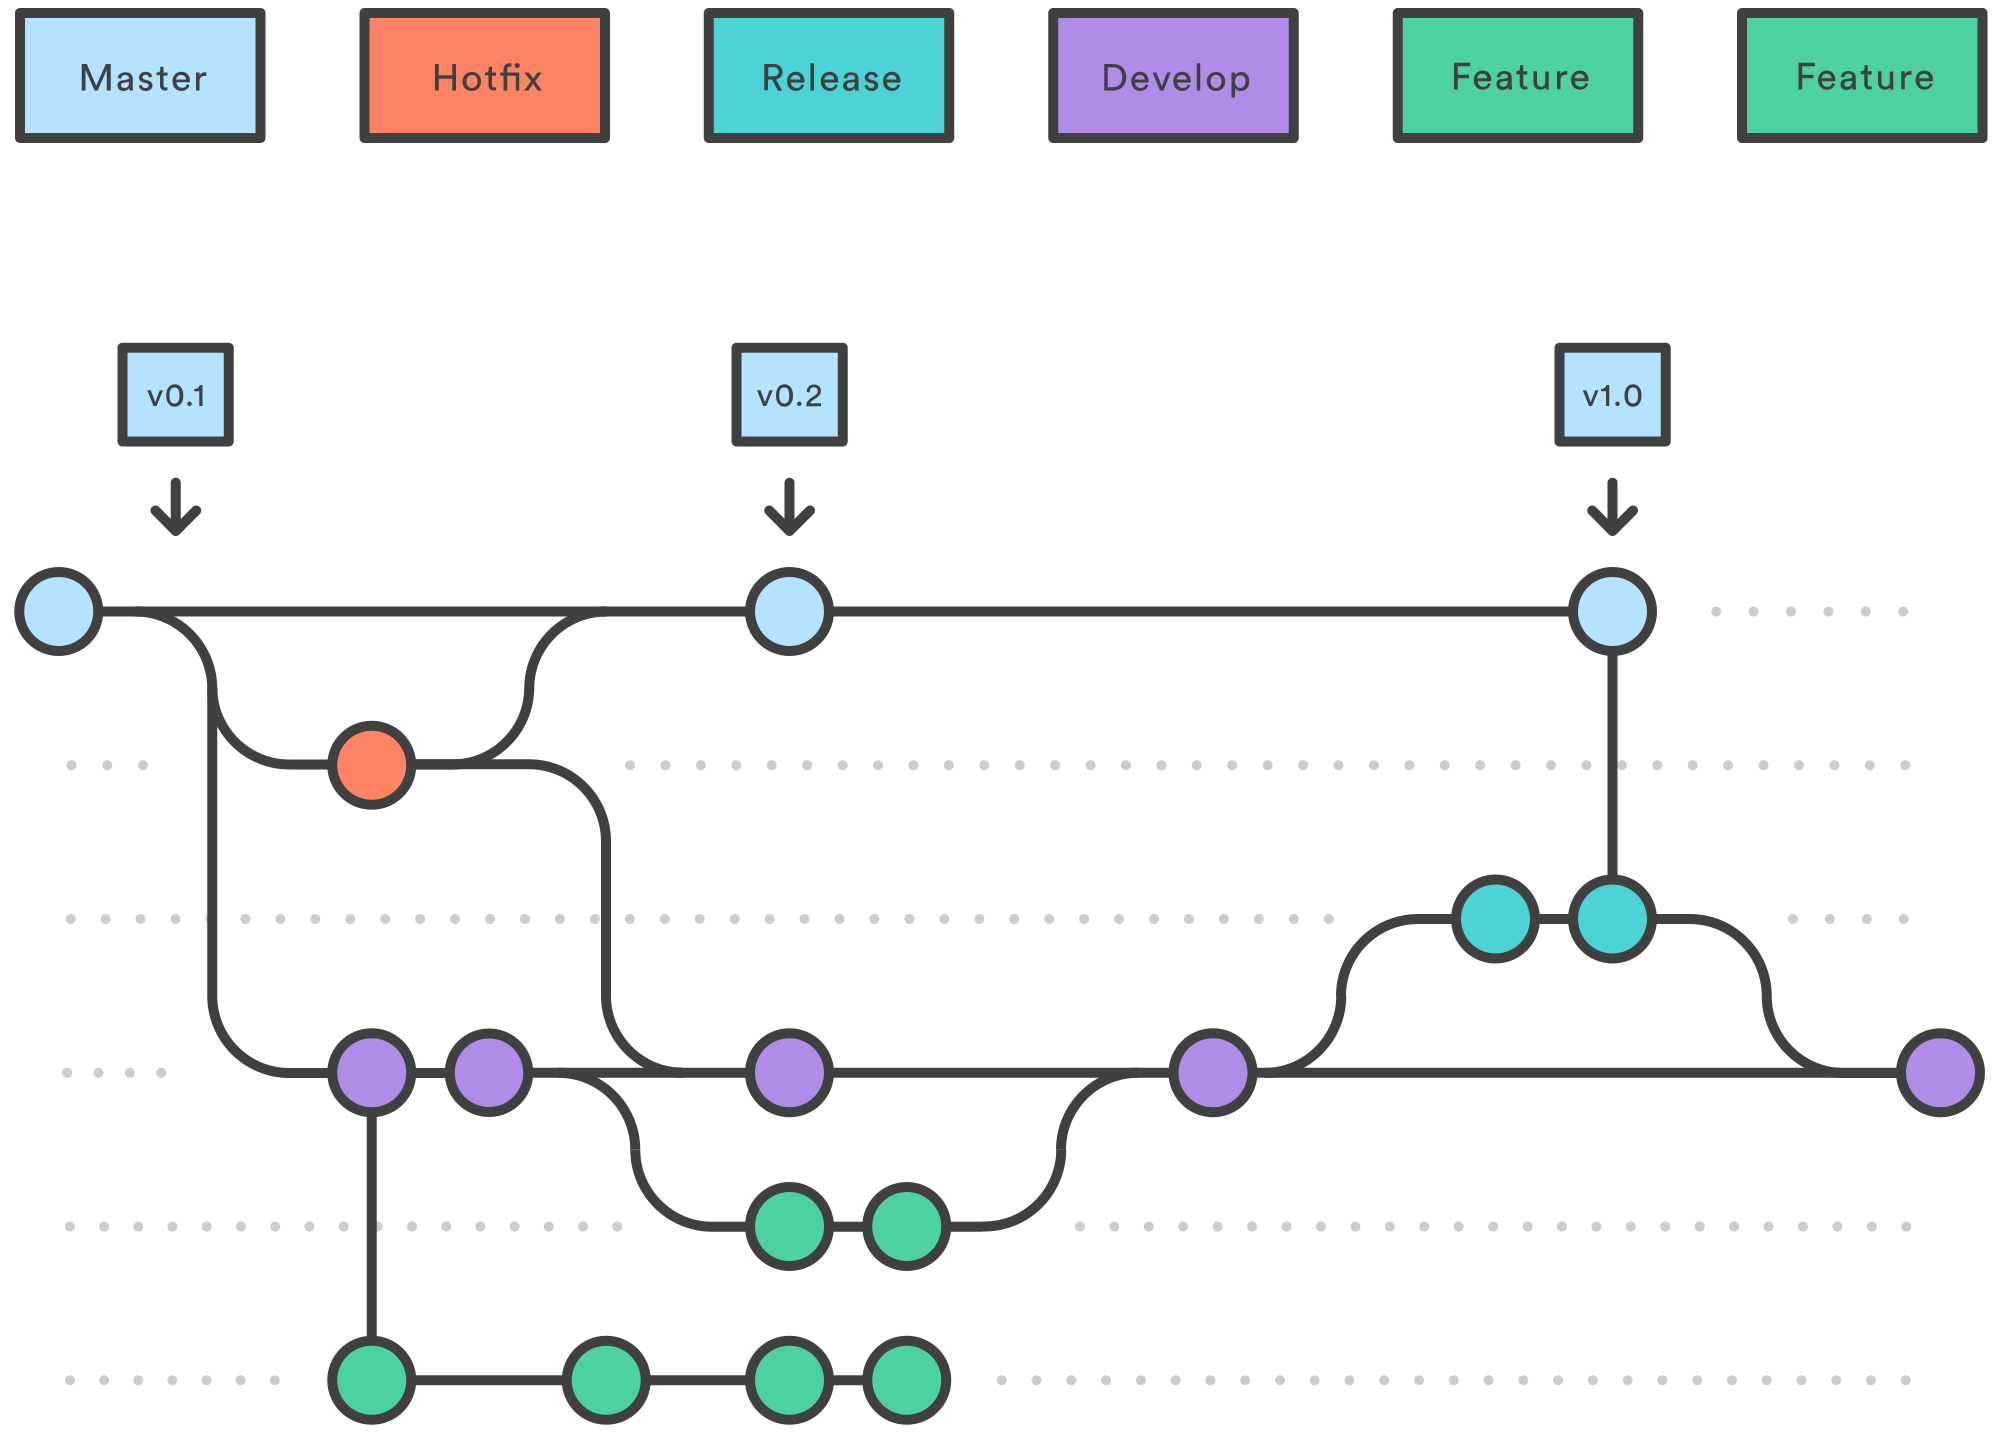
\includegraphics[width=\columnwidth]{img/gitflow}
	\caption[Gitflow]{Gitflow\footnotemark}
\end{figure}
\footnotetext{\cite{atlassian2020}}

Der Gitflow-Workflow definiert ein strenges Branching-Model und gibt jedem Typ von Branch (lediglich differenziert durch ihre Namen) eine spezifische Rolle. \code{Master} wird verwendet, um die Release-History festzuhalten. Hier finden sich Versionen des Projekts, die lauffähig sind und für sich alleine stehen (können). \code{Development} fungiert ähnlich wie \code{Master}, nur enthält es die gesamte Entwicklungshistorie des Projekts. Nun kommen die sogenannten \code{Feature}-Branches ins Spiel. Benannt werden Features hierarchisch. Im Projekt werden folgende zwei Gruppen verwendet: 

\begin{minipage}{\textwidth}
\texttt{feature/\textbf{backend}/<konkretes-feature>}

\texttt{feature/\textbf{frontend}/<konkretes-feature>}
\end{minipage}

Jedes Feature wird einem Verantwortlichen zugeteilt und wird meist auch von diesem bearbeitet. Sobald ein Feature fertig ist, wird es in \code{Development} zusammengeführt. Somit werden die Abstände zwischen Zusammenführungen verringert und der Arbeitsablauf wird einfacher. Schließlich gibt es auch noch einen Hotfix-Branch für dringende Änderungen.

Im Laufe der Entwicklung haben sich die Vorteile dieser Herangehensweise für das Team deutlich gezeigt. Unterschiedliche Features konnten, nachdem eine grundlegende Programmarchitektur umgesetzt worden ist, meist ohne Probleme zusammengeführt werden. 

\para{Nutzung von Stack für Notation [Schwenke]}

Der Taschenrechner soll als Eingabelogik für die Anwendung von Operationen die umgekehrte polnische Notation verwenden. Hierbei werden immer zunächst die Operanden und im Anschluss daran die darauf auszuführenden Operatoren angegeben. Dieser Ansatz ermöglicht eine stapelbasierte Abarbeitung. 

Stacks werden, wie von den meisten Programmiersprachen, auch in Java in der Standardbibliothek unterstützt. Mit dabei sind Methoden wie \code{push} (für das Ablegen eines Objekts auf dem Stapel), \code{pop} (für das Entfernen und die Wiedergabe eines Objekts auf dem Stapel), \code{peek} (für die Wiedergabe ohne Entfernen eines Objekts auf dem Stapel) und \code{empty} (für das Leeren des Stapels). 

Jedoch müssen hierbei die besonderen Anforderungen des Taschenrechners beachtet werden. Operanden können von gänzlich unterschiedlichem Typus sein, zum Beispiel eine einfache Dezimalzahl oder auch ein Tupel, und viele Operationen benötigen mehr als die ersten (maximal zwei) Operanden auf dem Stack. Möchte man Elemente vom Stapel entfernen, kann man \code{pop} mehrmals aufrufen. Aufwändiger hingegen wird es bei \code{peek}. Möchte man mehrere Elemente vom Stapel einsehen ohne diese zu entfernen, muss man bei der Arbeit mit dem vorhandenen Stack einen weiteren bereithalten, nur um zwischengespeicherte Elemente lagern zu können. Anders ist es nicht möglich \code{peek} auf mehrere Elemente gleichzeitig anzuwenden. Gerade das ist aber bei der App notwendig. Weitere Methoden, die bei der umgekehrten polnischen Notation oft benötigt werden, aber nicht implementiert sind, sind \code{reverse} (für die Vertauschung der ersten zwei Elemente auf dem Stack, was wichtig für nicht-kommutative Operationen ist), \code{rollUp} (das unterste Elemente wird an den ersten Platz geschoben, das erste Element an den zweiten Platz usw.) und \code{rollDown} (das unterste Elemente wird an den ersten Platz geschoben, das erste Element an den zweiten Platz usw.).

Aufgrund dessen soll für dieses Projekt ein eigener Stapel implementiert werden. Dieser soll die zuvor genannten Funktionen mit unterschiedlichen Parametertypen unterstützen. Dabei ist darauf zu achten, dass die Programmierung generisch erfolgt und das Stack nicht nur alle Typen von Operanden unterstützt, sondern auch für gänzlich andere Klassenbäume in der App verwendet werden kann.

\para{Ansatz der Kalkulationsorchestrierung [Schwenke]}

Die App soll den Umgang mit unterschiedlichen Operanden-Typen beherrschen. Die Addition zweier Matrizen funktioniert anders als die Addition von zwei einfachen Dezimalzahlen. Java verfügt nativ weder über die entsprechenden Operanden noch über die Methoden für die Kalkulation. Auch die ausgewählte Bibliothek ist nicht ohne weiteres in der Lage Operationen auf alle Kombinationen von Operanden im folgenden Format einheitlich anzuwenden:

\begin{figure}[bht]
	\begin{lstlisting}[caption=Konzept für Nutzung generischer Schnittstelle, label=list:konzept-fuer-nutzung-generischer-schnittstelle]
	Operation.mit(matrixOperand, dezimalOperand, dezimalOperand)
	\end{lstlisting}    
\end{figure}

Einheitlichkeit ist notwendig, damit im Frontend der Applikation keine Logik vorhanden sein muss, die entscheidet wie genau (auf Basis der Operanden-Typen) eine Operation umgesetzt wird. Deswegen muss eine einfache Schnittstelle entwickelt werden, die für den Nutzer nur zwei Drehschrauben bereitstellt. Dies ist zunächst die Auswahl der gewünschten Operation. Das kann z.B. das Symbol \code{+} als übliches Zeichen für Addition sein. Anschließend wird eine Reihe von Operanden übergeben. Dieser Aufruf sollte schließlich das Ergebnis in Form eines Operanden zurückgeben. Im Fall der Addition einer Matrix mit einer rationalen Zahl wäre dies wiederrum eine Matrix. Die korrekte Kalkulation soll also dynamisch bestimmt werden. Wichtig zu klären ist hier auch das Verhalten im Falle eines Fehlschlags. Nicht alle Kombinationen von Operanden können unterstützt werden. Die Verwendung von \textit{Optionals} (ein \code{Optional} ist ein Objekt, das man sich als Datenbehälter vorstellen kann, der entweder einen Wert enthält oder leer – aber nicht \code{null} sein kann) bietet sich hier zwar an, wird jedoch von Java in der verwendeten Android API-Version nicht unterstützt. Deswegen ist hier geplant sogenannte \textit{checked Exceptions} zu verwenden. Diese müssen bei der Verwendung explizit aufgefangen und weiterverarbeitet werden. Die Abbildung einer Operanden-Kombination auf die entsprechende konkrete Kalkulationsmethode muss dementsprechend zur Laufzeit des Programms erfolgen. Ein solches Mapping ist in Java nur mithilfe des Reflection-Pakets möglich. Reflektion ermöglicht den Einblick in ein Objekt (neben der Nutzung des Punkt-Operators) in eine Klasse. Zum Beispiel kann man eine Methode anhand einer Kombination von Parametertypen finden und aufrufen. Es ist geplant diesen Ansatz für die Orchestrierung der Kalkulationen in der App zu verwenden. Auch ist es nicht notwendig nur eine vordefinierte Anzahl an Argumente anzunehmen. So kann es sinnvoll sein, dass eine Methode zur Erstellung eines Tupels eine beliebige Anzahl an Operanden annimmt. Auch das lässt sich mit Reflektion umsetzen.

Der große Vorteil dabei ist, dass nirgendwo explizit in einer Abfrage entschieden werden muss, welche Kombination von Operanden an welche Methode weitergeleitet werden soll. Die Zuordnung erfolgt rein über die Deklaration der Parametertypen in der Methode selbst. Das macht das Ändern und Erweitern der Rechenfunktionalitäten einfach. Es muss lediglich die entsprechende Klasse herausgesucht und eine Methode im korrekten Format hinzugefügt werden. 

\para{Nutzung von Stack für Notation [Schwenke]}

Der Taschenrechner soll als Eingabelogik für die Anwendung von Operationen die umgekehrte polnische Notation verwenden. Hierbei werden immer zunächst die Operanden und im Anschluss daran die darauf auszuführenden Operatoren angegeben. Dieser Ansatz ermöglicht eine stapelbasierte Abarbeitung. 

Stacks werden, wie von den meisten Programmiersprachen, auch in Java in der Standardbibliothek unterstützt. Mit dabei sind Methoden wie \code{push} (für das Ablegen eines Objekts auf dem Stapel), \code{pop} (für das Entfernen und die Wiedergabe eines Objekts auf dem Stapel), \code{peek} (für die Wiedergabe ohne Entfernen eines Objekts auf dem Stapel) und \code{empty} (für das Leeren des Stapels). 

Jedoch müssen hierbei die besonderen Anforderungen des Taschenrechners beachtet werden. Operanden können von gänzlich unterschiedlichem Typus sein, zum Beispiel eine einfache Dezimalzahl oder auch ein Tupel, und viele Operationen benötigen mehr als die ersten (maximal zwei) Operanden auf dem Stack. Möchte man Elemente vom Stapel entfernen, kann man \code{pop} mehrmals aufrufen. Aufwändiger hingegen wird es bei \code{peek}. Möchte man mehrere Elemente vom Stapel einsehen ohne diese zu entfernen, muss man bei der Arbeit mit dem vorhandenen Stack einen weiteren bereithalten, nur um zwischengespeicherte Elemente lagern zu können. Anders ist es nicht möglich \code{peek} auf mehrere Elemente gleichzeitig anzuwenden. Gerade das ist aber bei der App notwendig. Weitere Methoden, die bei der umgekehrten polnischen Notation oft benötigt werden, aber nicht implementiert sind, sind \code{reverse} (für die Vertauschung der ersten zwei Elemente auf dem Stack, was wichtig für nicht-kommutative Operationen ist), \code{rollUp} (das unterste Elemente wird an den ersten Platz geschoben, das erste Element an den zweiten Platz usw.) und \code{rollDown} (das unterste Elemente wird an den ersten Platz geschoben, das erste Element an den zweiten Platz usw.).

Aufgrund dessen soll für dieses Projekt ein eigener Stapel implementiert werden. Dieser soll die zuvor genannten Funktionen mit unterschiedlichen Parametertypen unterstützen. Dabei ist darauf zu achten, dass die Programmierung generisch erfolgt und das Stack nicht nur alle Typen von Operanden unterstützt, sondern auch für gänzlich andere Klassenbäume in der App verwendet werden kann.

\para{Ansatz der Kalkulationsorchestrierung [Schwenke]}

Die App soll den Umgang mit unterschiedlichen Operanden-Typen beherrschen. Die Addition zweier Matrizen funktioniert anders als die Addition von zwei einfachen Dezimalzahlen. Java verfügt nativ weder über die entsprechenden Operanden noch über die Methoden für die Kalkulation. Auch die ausgewählte Bibliothek ist nicht ohne weiteres in der Lage Operationen auf alle Kombinationen von Operanden im folgenden Format einheitlich anzuwenden:

\begin{figure}[bht]
	\begin{lstlisting}[caption=Konzept für Nutzung generischer Schnittstelle, label=list:konzept-fuer-nutzung-generischer-schnittstelle]
	Operation.mit(matrixOperand, dezimalOperand, dezimalOperand)
	\end{lstlisting}    
\end{figure}

Einheitlichkeit ist notwendig, damit im Frontend der Applikation keine Logik vorhanden sein muss, die entscheidet wie genau (auf Basis der Operanden-Typen) eine Operation umgesetzt wird. Deswegen muss eine einfache Schnittstelle entwickelt werden, die für den Nutzer nur zwei Drehschrauben bereitstellt. Dies ist zunächst die Auswahl der gewünschten Operation. Das kann z.B. das Symbol \code{+} als übliches Zeichen für Addition sein. Anschließend wird eine Reihe von Operanden übergeben. Dieser Aufruf sollte schließlich das Ergebnis in Form eines Operanden zurückgeben. Im Fall der Addition einer Matrix mit einer rationalen Zahl wäre dies wiederrum eine Matrix. Die korrekte Kalkulation soll also dynamisch bestimmt werden. Wichtig zu klären ist hier auch das Verhalten im Falle eines Fehlschlags. Nicht alle Kombinationen von Operanden können unterstützt werden. Die Verwendung von \textit{Optionals} (ein \code{Optional} ist ein Objekt, das man sich als Datenbehälter vorstellen kann, der entweder einen Wert enthält oder leer – aber nicht \code{null} sein kann) bietet sich hier zwar an, wird jedoch von Java in der verwendeten Android API-Version nicht unterstützt. Deswegen ist hier geplant sogenannte \textit{checked Exceptions} zu verwenden. Diese müssen bei der Verwendung explizit aufgefangen und weiterverarbeitet werden. Die Abbildung einer Operanden-Kombination auf die entsprechende konkrete Kalkulationsmethode muss dementsprechend zur Laufzeit des Programms erfolgen. Ein solches Mapping ist in Java nur mithilfe des Reflection-Pakets möglich. Reflektion ermöglicht den Einblick in ein Objekt (neben der Nutzung des Punkt-Operators) in eine Klasse. Zum Beispiel kann man eine Methode anhand einer Kombination von Parametertypen finden und aufrufen. Es ist geplant diesen Ansatz für die Orchestrierung der Kalkulationen in der App zu verwenden. Auch ist es nicht notwendig nur eine vordefinierte Anzahl an Argumente anzunehmen. So kann es sinnvoll sein, dass eine Methode zur Erstellung eines Tupels eine beliebige Anzahl an Operanden annimmt. Auch das lässt sich mit Reflektion umsetzen.

Der große Vorteil dabei ist, dass nirgendwo explizit in einer Abfrage entschieden werden muss, welche Kombination von Operanden an welche Methode weitergeleitet werden soll. Die Zuordnung erfolgt rein über die Deklaration der Parametertypen in der Methode selbst. Das macht das Ändern und Erweitern der Rechenfunktionalitäten einfach. Es muss lediglich die entsprechende Klasse herausgesucht und eine Methode im korrekten Format hinzugefügt werden. 

Zu entscheiden ist ebenfalls, ob das Gros der Rechenmethoden innerhalb der jeweiligen Operanden-Klassen oder dedizierten Klassen für die Kalkulation angesiedelt sind. Die erste Option hat neben der stärkeren Objektorientierung den Vorteil, dass immer klar ist, dass eine Methode mit den übergebenen Argumenten auf dem jeweiligen Objekt ausgeführt wird. Andererseits erhöht dies die Komplexität der Operanden-Klassen deutlich. Unterstützt man wie geplant 5 bis 7 dedizierte Typen von Operanden und 10 Kalkulationsarten, muss jede Klasse potenziell dutzende Methoden für die Rechnung enthalten. Die andere, und bevorzugte Option, ist die Auslagerung der Kalkulationsmethoden in eigenständige Klassen. Dies reduziert zwar nicht die Anzahl benötigter Methoden, isoliert die Rechenlogik jedoch in Klassen. Innerhalb dieser Klassen wird prozedural programmiert.  Eine typische Charakteristik von Objekten und deren Methoden ist \textit{Mutability}. Eine Methode bekommt ein Objekt und kann dieses verändern. Dies kann Testen unter Umständen aufwändiger gestalten. Durch Isolierung der Rechnungen in eigenen Klassen kann hingegen sichergestellt werden, dass jede Methode \textit{immutable}, also unveränderlich, ist. Das macht das Schreiben von Tests einfach. In Java kann Immutability durch die Verwendung von Annotationen sichergestellt werden. 

